\chapter{PmodCLP}

Der PmodCLP besteht aus einem Samsung KS0066 LCD Controller und einem Sunlike LCD Panel, worüber Informationen dargestellt werden können {lcd-desc}. Es ist möglich 32 Positionen auf dem 16x2 LCD Panel zu nutzen. Pro Position werden die Zeichen dabei mit einer Auflösung von 5x8 angezeigt. \newline

Das System besteht im Wesentlichen aus drei Komponenten. Der character-generator ROM (CGROM) hält 192 vordefinierte Zeichen, darunter 93 ASCII Charaktere. Anschaulich gesehen können die Zeichen über eine matrixartige Struktur indiziert werden, welche im Datenblatt festgelegt ist. Neben den nicht-volatilen Daten im CGROM ist es möglich bis zu 8 eigene Zeichen volatil im character-generator RAM (CGRAM) zu halten. Um nun Zeichen aus diesen beiden Repositories auf dem Panel anzeigen zu können, gibt es den data RAM (DDRAM). Hier können bis zu 80 Zeichencodes gespeichert werden. Er fungiert als Indexspeicher für Daten innerhalb des CGROM oder CGRAM. Wird ein Index aus der matrixartigen Struktur in den DDRAM geladen, erscheint das entsprechende Zeichen auf dem Display. \newline

Das Display selbst verfügt über 2 Zeilen á 16 Positionen. Insgesamt stehen jedoch nicht 32 Speicherplätze zur Verfügung, sondern 39, um beispielsweise Scrolling zu verwenden. \newline

Wichtige Schnittstellen des Samsung KS0066 LCD Controller sind

\begin{itemize}
    \item \textit{DB4-DB7}: Datenbits im Nibble-Mode zur Codierung von Befehlen/Zeichen
    \item \textit{RS (Register Select)}: High für Daten, Low für Instruktionen
    \item \textit{RW (Read/Write)}: High = Read, Low = Write
    \item \textit{E (Enable)}: High für Read, Falling Edge für Write
\end{itemize}

Um diese nutzen zu können wird folgendes Mapping auf dem FPGA hinterlegt:\newline

\begin{lstlisting}[language=bash,caption={Pin-Zuordnung im Constraints-File},breaklines=true,captionpos=b,basicstyle=\footnotesize\ttfamily,
    label={lst:fpga_pins}]
set_property -dict {PACKAGE_PIN D13 IOSTANDARD LVCMOS33}[get_ports{clp_db_tri_io[4]}];#db04
set_property -dict {PACKAGE_PIN B18 IOSTANDARD LVCMOS33}[get_ports{clp_db_tri_io[5]}];#db05
set_property -dict {PACKAGE_PIN A18 IOSTANDARD LVCMOS33}[get_ports{clp_db_tri_io[6]}];#db06
set_property -dict {PACKAGE_PIN K16 IOSTANDARD LVCMOS33}[get_ports{clp_db_tri_io[7]}];#db07
set_property -dict {PACKAGE_PIN E2 IOSTANDARD LVCMOS33}[get_ports{clp_cb_tri_o[0]}];  #lcd_rs
set_property -dict {PACKAGE_PIN D2 IOSTANDARD LVCMOS33}[get_ports{clp_cb_tri_o[1]}];  #lcd_rw
set_property -dict {PACKAGE_PIN H2 IOSTANDARD LVCMOS33}[get_ports{clp_cb_tri_o[2]}];  #lcd_e
\end{lstlisting}

Die Zuordung in Aufzählung \ref{lst:fpga_pins} greift auf zwei Header des PmodCLP-Boards zurück. Die Daten-Bits db04-db07 sind an die untere Hälfte des Headers J1 gebunden. Die Steuersignale Register Select, Read/Write und Enable hingegen an Header J2.

\section{Ansatz Custom IP}

Im ersten Schritt soll die IP funktional fertiggestellt werden. Sie soll dabei mittels Polling eingesetzt werden. Sobald die Funktionalität des Gesamtsystems vollumfänglich gegeben ist, wird anstatt Polling über Interrupts kommuniziert.\newline

Das Projektteam hat sich auf folgenden Entwurf geeinigt:

\begin{itemize}
    \item \textit{Submodul 1}: LCD-Controller (FSM) \newline
    Mittels einer FSM wird aus den Registern, welche von Microprozessor gesetzt werden können, der Befehl interpretiert.
    \item \textit{Submodul 2}: Timing Controller \newline
    Dies kann bspw. mit einem Zähler, der als Timer in Abhängigkeit vom Systemtakt fungiert, umgesetzt werden.
    Diverse Statusflags sollen den aktuellen Stand zeigen.\newline
    \begin{figure}[h!]
        \centering
        \begin{minipage}{0.15\textwidth}
            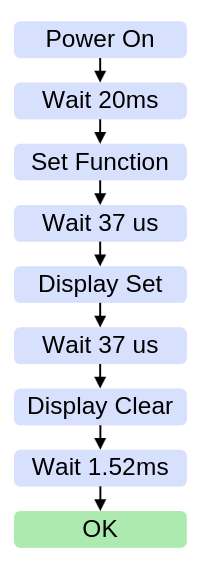
\includegraphics[width=\linewidth]{./images/lcd_timing.png} % replace with your image filename
        \end{minipage}
        \caption{Startup Sequence}
        \label{fig:startup_sequence}
    \end{figure}
    \newline
    Graphik \ref{fig:startup_sequence} zeigt die Initialisierung des Displays und die damit verbundenen Timing-Anforderungen.
    \item \textit{Submodul 3}: Character Transfomer  \newline
    Die vom Sensor erhaltenen Werte müssen in entsprechende Werte, die auf dem Display dargestellt werden können, umgewandelt werden. Eine lookup-table soll hier Abhilfe schaffen.
    \item \textit{Submodul 4}: Memory Mapping  \newline
    Dieses Submodul soll eines standardisierte und zuverlässige DDRAM-Adressierung garantieren. Dabei muss das Display-Layout (16x2) beachtet werden. Mögliche Erweiterungen, wie bspw. Scrolling, sollen bei der Implementierung bereits stets bedacht werden.
    \item \textit{Submodul 5}: LCD-Communication Interface  \newline
    Hier werden die Daten in die entsprechenden Register geschrieben, um die Werte anschließend auf dem Display darzustellen.
    \item \textit{Submodul 6}: AXI Slave Interface  \newline
    Nachdem die Zuverlässigkeit der IP mittels Tests sichergestellt wurde, soll die IP an den internen Systembus (AXI) angebunden werden.
\end{itemize}

Das Registermapping wurde in Anlehnung an \textit{at\_doc.pdf} aus \textit{02b\_tut\_vhdl\_v03} erstellt.

\section{Registermapping}

\subsection{I/Os}
\begin{longtable}{|p{2.5cm}|p{1cm}|p{2cm}|p{9cm}|}
\hline
\textbf{Signal Name} & \textbf{I/O} & \textbf{Initial State} & \textbf{Description} \\
\hline
ap\_clk(s00\_axi\_aclk) & I & NA & AXI Clock \\
\hline
ap\_rst\_n (s00\_axi\_aresetn) & I & NA & AXI Reset, active-Low \\
\hline
s\_axi\_control* (s00\_axi*) & NA & NA & AXI4-Lite Slave Interface signals \\
\hline
interrupt & I & 0x0 & Indicates that the condition for an interrupt has occurred. (new sensor value available)
\newline 0 = No interrupt has occurred
\newline 1 = Interrupt has occurred \\
\hline
sensor\_val\_in & I & 0xFF & Input value from PmodMAXSONAR \\
\hline
db4\_7\_out & O & 0xFF & 4 data bits, necessary in nibble mode. \\
\hline
register\_select\_out & O & 0x1 & Register Select: High for Data Transfer, Low for Instruction Transfer \\
\hline
read\_write\_out & O & 0x1 & Read/Write signal: High for Read mode, Low for Write mode \\
\hline
read\_write\_enable\_out & O & 0x1 & Read/Write Enable: High for Read, falling edge writes data \\
\hline
\caption{PmodCLP Überblick I/O}
\end{longtable}

\subsection{Registerbereich}
% PmodCLP Controller Register Mapping in LaTeX with longtables
% Register Space Overview Table
\begin{longtable}{|p{3cm}|p{3cm}|p{8cm}|}
    \hline
    \textbf{Address Offset} & \textbf{Register Name} & \textbf{Description} \\
    \hline
    \endfirsthead
    \hline
    \textbf{Address Offset} & \textbf{Register Name} & \textbf{Description} \\
    \hline
    \endhead
    \hline \multicolumn{3}{|r|}{{Continued on next page}} \\ \hline
    \endfoot
    \hline
    \endlastfoot
    
    0x00 & GCSR & General/Global Control and Status Register \\
    \hline
    0x04 & GIER & Global Interrupt Enable Register \\
    \hline
    0x08 & IPIER & IP Interrupt Enable Register \\
    \hline
    0x0C & IPISR & IP Interrupt Status Register \\
    \hline
    0x10 & IDR & ID Register \\
    \hline
    0x14 & VERR & Version Register \\
    \hline
    0x18 & SCSR0 & Special Control and Status Register \\
    \hline
    0x1C & CDR & Character Data Register \\
    \hline
    \caption{PmodCLP Controller Register Space Overview}
    \label{tab:register_overview}
    \end{longtable}
    
    % GCSR Register Table
    \begin{longtable}{|p{1cm}|p{3cm}|p{2cm}|p{2cm}|p{6cm}|}
    \hline
    \textbf{Bit} & \textbf{Name} & \textbf{Access Type} & \textbf{Reset Value} & \textbf{Description} \\
    \hline
    \endfirsthead
    \hline
    \textbf{Bit} & \textbf{Name} & \textbf{Access Type} & \textbf{Reset Value} & \textbf{Description} \\
    \hline
    \endhead
    \hline \multicolumn{5}{|r|}{{Continued on next page}} \\ \hline
    \endfoot
    \hline
    \endlastfoot
    
    \multicolumn{5}{|c|}{\textbf{0x00 GCSR - General/Global Control and Status Register}} \\
    \hline
    0 & ap\_start & R/W & 0 & Asserted when the kernel can start processing data. Cleared on handshake with ap\_done being asserted. \\
    \hline
    1 & ap\_done & R & 0 & Asserted when the kernel has completed initialization operation. Cleared on read. \\
    \hline
    2 & ap\_idle & R & 0 & Asserted when the kernel is idle. \\
    \hline
    3 & \textit{reserved (ap\_ready)} & R & 0 & Asserted by the kernel when it is ready to accept new data (used only by AP\_CTRL\_CHAIN) \\
    \hline
    4 & \textit{reserved (ap\_continue)} & R/W & 0 & Asserted by the XRT to allow kernel keep running (used only by AP\_CTRL\_CHAIN) \\
    \hline
    5:6 & reserved & & & \\
    \hline
    7 & auto\_restart & R/W & 0 & Used to enable automatic kernel restart. This bit determines whether the display reloads the last sensor value and continues running or clears the display. \\
    \hline
    8 & lcd\_initialized & R & 0 & Indicates the LCD has been properly initialized and is ready for commands. \\
    \hline
    9 & display\_busy & R & 0 & Indicates the display is currently processing a command. \\
    \hline
    10 & error\_flag & R & 0 & Indicates an error occurred during last operation. \\
    \hline
    31:11 & reserved & & & \\
    \caption{General/Global Control and Status Register (GCSR)}
    \label{tab:gcsr}
    \end{longtable}
    
    % GIER Register Table
    \begin{longtable}{|p{1cm}|p{3cm}|p{2cm}|p{2cm}|p{6cm}|}
    \hline
    \textbf{Bit} & \textbf{Name} & \textbf{Access Type} & \textbf{Reset Value} & \textbf{Description} \\
    \hline
    \endfirsthead
    \hline
    \textbf{Bit} & \textbf{Name} & \textbf{Access Type} & \textbf{Reset Value} & \textbf{Description} \\
    \hline
    \endhead
    \hline \multicolumn{5}{|r|}{{Continued on next page}} \\ \hline
    \endfoot
    \hline
    \endlastfoot
    
    \multicolumn{5}{|c|}{\textbf{0x04 GIER - Global Interrupt Enable Register}} \\
    \hline
    0 & gie & R/W & 0 & When asserted, along with the IP Interrupt Enable bit, the interrupt is enabled. \\
    \hline
    31:1 & reserved & & & \\
    \hline
    \caption{Global Interrupt Enable Register (GIER)}
    \label{tab:gier}
    \end{longtable}
    
    % IPIER Register Table
    \begin{longtable}{|p{1cm}|p{3cm}|p{2cm}|p{2cm}|p{6cm}|}
    \hline
    \textbf{Bit} & \textbf{Name} & \textbf{Access Type} & \textbf{Reset Value} & \textbf{Description} \\
    \hline
    \endfirsthead
    \hline
    \textbf{Bit} & \textbf{Name} & \textbf{Access Type} & \textbf{Reset Value} & \textbf{Description} \\
    \hline
    \endhead
    \hline \multicolumn{5}{|r|}{{Continued on next page}} \\ \hline
    \endfoot
    \hline
    \endlastfoot
    
    \multicolumn{5}{|c|}{\textbf{0x08 IPIER - IP Interrupt Enable Register}} \\
    \hline
    0 & ipie & R/W & 0 & When asserted, along with Global Interrupt Enable bit, the interrupt is enabled. (default: uses the internal ap\_done signal to trigger an interrupt) \\
    \hline
    31:1 & reserved & & & \\
    \hline
    \caption{IP Interrupt Enable Register (IPIER)}
    \label{tab:ipier}
    \end{longtable}
    
    % IPISR Register Table
    \begin{longtable}{|p{1cm}|p{3cm}|p{2cm}|p{2cm}|p{6cm}|}
    \hline
    \textbf{Bit} & \textbf{Name} & \textbf{Access Type} & \textbf{Reset Value} & \textbf{Description} \\
    \hline
    \endfirsthead
    \hline
    \textbf{Bit} & \textbf{Name} & \textbf{Access Type} & \textbf{Reset Value} & \textbf{Description} \\
    \hline
    \endhead
    \hline \multicolumn{5}{|r|}{{Continued on next page}} \\ \hline
    \endfoot
    \hline
    \endlastfoot
    
    \multicolumn{5}{|c|}{\textbf{0x0C IPISR - IP Interrupt Status Register}} \\
    \hline
    0 & ipis & R/W & 0 & Toggle on write. (write 1 to clear(W1C)) \\
    \hline
    31:1 & reserved & & & \\
    \hline
    \caption{IP Interrupt Status Register (IPISR)}
    \label{tab:ipisr}
    \end{longtable}
    
    % IDR Register Table
    \begin{longtable}{|p{1cm}|p{3cm}|p{2cm}|p{2cm}|p{6cm}|}
    \hline
    \textbf{Bit} & \textbf{Name} & \textbf{Access Type} & \textbf{Reset Value} & \textbf{Description} \\
    \hline
    \endfirsthead
    \hline
    \textbf{Bit} & \textbf{Name} & \textbf{Access Type} & \textbf{Reset Value} & \textbf{Description} \\
    \hline
    \endhead
    \hline \multicolumn{5}{|r|}{{Continued on next page}} \\ \hline
    \endfoot
    \hline
    \endlastfoot
    
    \multicolumn{5}{|c|}{\textbf{0x10 IDR - ID Register}} \\
    \hline
    31:0 & ID & R & 0x80010744 & Distinct ID for PmodCLP Controller \\
    \hline
    \caption{ID Register (IDR)}
    \label{tab:idr}
    \end{longtable}
    
    % VERR Register Table
    \begin{longtable}{|p{1cm}|p{3cm}|p{2cm}|p{2cm}|p{6cm}|}
    \hline
    \textbf{Bit} & \textbf{Name} & \textbf{Access Type} & \textbf{Reset Value} & \textbf{Description} \\
    \hline
    \endfirsthead
    \hline
    \textbf{Bit} & \textbf{Name} & \textbf{Access Type} & \textbf{Reset Value} & \textbf{Description} \\
    \hline
    \endhead
    \hline \multicolumn{5}{|r|}{{Continued on next page}} \\ \hline
    \endfoot
    \hline
    \endlastfoot
    
    \multicolumn{5}{|c|}{\textbf{0x14 VERR - Version Register}} \\
    \hline
    31:0 & VER & R & 0x80001000 & Version \\
    \hline
    \caption{Version Register (VERR)}
    \label{tab:verr}
    \end{longtable}
    
    % SCSR0 Register Table
    \begin{longtable}{|p{1cm}|p{3cm}|p{2cm}|p{2cm}|p{6cm}|}
    \hline
    \textbf{Bit} & \textbf{Name} & \textbf{Access Type} & \textbf{Reset Value} & \textbf{Description} \\
    \hline
    \endfirsthead
    \hline
    \textbf{Bit} & \textbf{Name} & \textbf{Access Type} & \textbf{Reset Value} & \textbf{Description} \\
    \hline
    \endhead
    \hline \multicolumn{5}{|r|}{{Continued on next page}} \\ \hline
    \endfoot
    \hline
    \endlastfoot
    
    \multicolumn{5}{|c|}{\textbf{0x18 SCSR0 - Special Control and Status Register}} \\
    \hline
    0 & lcd\_enable & R/W & 0 & Master enable for LCD display (0 = disabled, 1 = enabled) \\
    \hline
    1 & clear\_display & R/W & 0 & Write 1 to clear the display, auto-clears when operation completes \\
    \hline
    2 & return\_home & R/W & 0 & Write 1 to return cursor to home position, auto-clears when operation completes \\
    \hline
    3 & cursor\_on & R/W & 0 & Enable cursor visibility (0 = off, 1 = on) \\
    \hline
    4 & cursor\_blink & R/W & 0 & Enable cursor blinking (0 = no blink, 1 = blink) \\
    \hline
    5 & display\_shift & R/W & 0 & Enable display shift (0 = no shift, 1 = shift) \\
    \hline
    6 & shift\_direction & R/W & 0 & Shift direction (0 = left, 1 = right) \\
    \hline
    7 & auto\_scroll & R/W & 0 & Enable automatic scrolling for long text \\
    \hline
    8 & reset\_lcd & R/W & 0 & Write 1 to reset LCD controller, auto-clears when operation completes \\
    \hline
    9 & busy\_flag & R & 0 & Indicates LCD controller is busy \\
    \hline
    10:15 & reserved & & & \\
    \hline
    23:16 & fsm\_state & R & 0 & Current state of LCD controller FSM (for debugging) \\
    \hline
    31:24 & error\_code & R & 0 & Error code if error\_flag is set in GCSR \\
    \hline
    \caption{Special Control and Status Register (SCSR0)}
    \label{tab:scsr0}
    \end{longtable}
    
    % CDR Register Table
    \begin{longtable}{|p{1cm}|p{3cm}|p{2cm}|p{2cm}|p{6cm}|}
    \hline
    \textbf{Bit} & \textbf{Name} & \textbf{Access Type} & \textbf{Reset Value} & \textbf{Description} \\
    \hline
    \endfirsthead
    \hline
    \textbf{Bit} & \textbf{Name} & \textbf{Access Type} & \textbf{Reset Value} & \textbf{Description} \\
    \hline
    \endhead
    \hline \multicolumn{5}{|r|}{{Continued on next page}} \\ \hline
    \endfoot
    \hline
    \endlastfoot
    
    \multicolumn{5}{|c|}{\textbf{0x1C CDR - Character Data Register}} \\
    \hline
    7:0 & char\_data & R/W & 0 & Character data to write to LCD \\
    \hline
    15:8 & char\_addr & R/W & 0 & DDRAM address for character (00H-27H for line 1, 40H-67H for line 2) \\
    \hline
    16 & write\_char & R/W & 0 & Write 1 to initiate character write to specified address \\
    \hline
    17 & read\_char & R/W & 0 & Write 1 to read character from specified address \\
    \hline
    31:18 & reserved & & & \\
    \hline
    \caption{Character Data Register (CDR)}
    \label{tab:cdr}
    \end{longtable}

TODO: Mit anderer Gruppe sprechen
- wie Austausch von Daten funktioniert, über Input/Register/? --> SDR??
- Formatting-Switch Inch/cm siehe FMR??


    % FMR Register Table
    \begin{longtable}{|p{1cm}|p{3cm}|p{2cm}|p{2cm}|p{6cm}|}
        \hline
        \textbf{Bit} & \textbf{Name} & \textbf{Access Type} & \textbf{Reset Value} & \textbf{Description} \\
        \hline
        \endfirsthead
        \hline
        \textbf{Bit} & \textbf{Name} & \textbf{Access Type} & \textbf{Reset Value} & \textbf{Description} \\
        \hline
        \endhead
        \hline \multicolumn{5}{|r|}{{Continued on next page}} \\ \hline
        \endfoot
        \hline
        \endlastfoot
        
        \multicolumn{5}{|c|}{\textbf{0x2C FMR - Format and Mode Register}} \\
        \hline
        0 & auto\_format & R/W & 0 & Enable automatic formatting of sensor data \\
        \hline
        1 & show\_units & R/W & 0 & Show measurement units alongside values \\
        \hline
        2 & leading\_zeros & R/W & 0 & Show leading zeros (0 = hide, 1 = show) \\
        \hline
        3 & fixed\_point & R/W & 0 & Enable fixed-point display format \\
        \hline
        7:4 & decimal\_places & R/W & 0 & Number of decimal places to display (0-8) \\
        \hline
        15:8 & display\_mode & R/W & 0 & Display mode selection (0 = raw, 1 = formatted, etc.) \\
        \hline
        31:16 & reserved & & & \\
        \hline
        \caption{Format and Mode Register (FMR)}
        \label{tab:fmr}
        \end{longtable}

    % SDR Register Table
    \begin{longtable}{|p{1cm}|p{3cm}|p{2cm}|p{2cm}|p{6cm}|}
        \hline
        \textbf{Bit} & \textbf{Name} & \textbf{Access Type} & \textbf{Reset Value} & \textbf{Description} \\
        \hline
        \endfirsthead
        \hline
        \textbf{Bit} & \textbf{Name} & \textbf{Access Type} & \textbf{Reset Value} & \textbf{Description} \\
        \hline
        \endhead
        \hline \multicolumn{5}{|r|}{{Continued on next page}} \\ \hline
        \endfoot
        \hline
        \endlastfoot
        
        \multicolumn{5}{|c|}{\textbf{0x30 SDR - Sensor Data Register}} \\
        \hline
        15:0 & sensor\_value & R/W & 0 & Raw sensor value from PmodMAXSONAR \\
        \hline
        23:16 & sensor\_status & R & 0 & Status code of sensor \\
        \hline
        31:24 & scaling\_factor & R/W & 0 & Scaling factor for sensor value display \\
        \hline
        \caption{Sensor Data Register (SDR)}
        \label{tab:sdr}
        \end{longtable}